% DO NOT COMPILE THIS FILE DIRECTLY!
% This is included by the other .tex files.

\begin{frame}[t,plain]
\titlepage
\end{frame}

\begin{frame}
 \frametitle{MISP features}
 \begin{itemize}
         \item MISP\footnote{\url{https://github.com/MISP/MISP}} is a threat information sharing free \& open source software.
         \item MISP has {\bf a host of functionalities} that assist users in creating, collaborating \& sharing threat information - e.g. flexible sharing groups, {\bf automatic correlation}, free-text import helper, event distribution \& proposals.
         \item Many export formats which support IDSes / IPSes (e.g. Suricata, Bro, Snort), SIEMs (eg CEF), Host scanners (e.g. OpenIOC, STIX, CSV, yara), analysis tools (e.g. Maltego), DNS policies (e.g. RPZ).
         \item A rich set of MISP modules\footnote{\url{https://www.github.com/MISP/misp-modules}} to add expansion, import and export functionalities.
 \end{itemize}
\end{frame}

\begin{frame}
 \frametitle{MISP and starting from a practical use-case}
 \begin{itemize}
         \item During a malware analysis workgroup in 2012, we discovered that we worked on the analysis of the same malware.
         \item We wanted to share information in an easy and automated way {\bf to avoid duplication of work}.
         \item Christophe Vandeplas (then working at the CERT for the Belgian MoD) showed us his work on a platform that later became MISP.
         \item A first version of the MISP Platform was used by the MALWG and {\bf the increasing feedback of users} helped us to build an improved platform.
         \item MISP is now {\bf a community-driven development}.
 \end{itemize}
\end{frame}

\begin{frame}
\frametitle{about CIRCL}
The Computer Incident Response Center Luxembourg (CIRCL) is a government-driven initiative designed to provide a systematic response facility to computer security threats and incidents. CIRCL is the CERT for the private sector, communes and non-governmental entities in Luxembourg and is operated by securitymadein.lu g.i.e.
\end{frame}

\begin{frame}
\frametitle{MISP and CIRCL}
\begin{itemize}
\item CIRCL is mandated by the Ministry of Economy and acting as the Luxembourg National CERT for private sector.
\item CIRCL leads the development of the Open Source MISP threat intelligence platform which is used by many military or intelligence communities, private companies, financial sector, National CERTs and LEAs globally.
\item {\bf CIRCL runs multiple large MISP communities performing active daily threat-intelligence sharing}.
\end{itemize}
        
\includegraphics{en_cef.png}
\end{frame}

\begin{frame}
\frametitle{MISP model of governance}
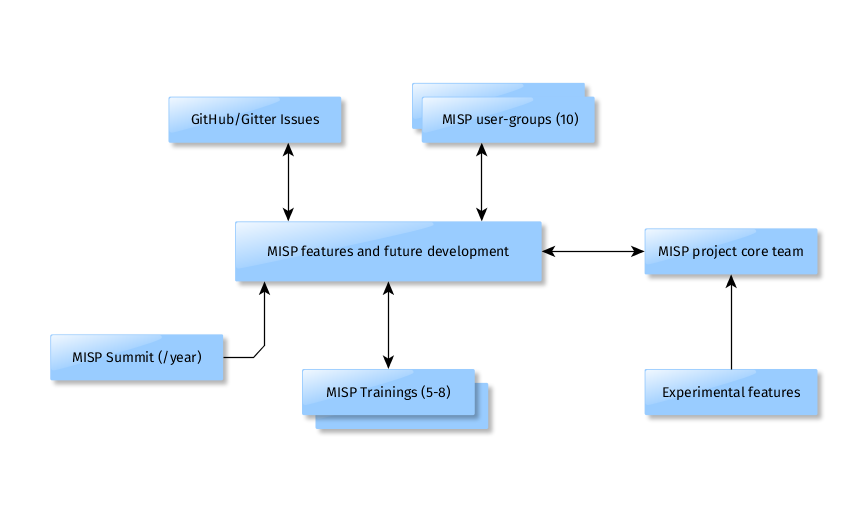
\includegraphics[scale=0.4]{governance.png}
\end{frame}

\begin{frame}
\frametitle{Development based on practical user feedback}
\begin{itemize}
\item There are many different types of users of an information sharing platform like MISP:
        \begin{itemize}
                \item {\bf Malware reversers} willing to share indicators of analysis with respective colleagues.
                \item {\bf Security analysts} searching, validating and using indicators in operational security.
                \item {\bf Intelligence analysts} gathering information about specific adversary groups.
                \item {\bf Law-enforcement} relying on indicators to support or bootstrap their DFIR cases.
                \item {\bf Risk analysis teams} willing to know about the new threats, likelyhood and occurences.
                \item {\bf Fraud analysts} willing to share financial indicators to detect financial frauds.
        \end{itemize}
\end{itemize}
\end{frame}

\begin{frame}
 \frametitle{Communities using MISP}
 \begin{itemize}
	 \item Communities are groups of users sharing within a set of common objectives/values.
	 \item CIRCL operates multiple MISP instances with a significant user base (more than 950 organizations with more than 2400 users).
     \item {\bf Trusted groups} running MISP communities in island mode (air gapped system) or partially connected mode.
	 \item {\bf Financial sector} (banks, ISACs, payment processing organizations) use MISP as a sharing mechanism.
	 \item {\bf Military and international organizations} (NATO, military CSIRTs, n/g CERTs,...).
	 \item {\bf Security vendors} running their own communities (e.g. Fidelis) or interfacing with MISP communities (e.g. OTX).
 \end{itemize}
\end{frame}

\begin{frame}
\frametitle{Many objectives from different user-groups}
        \begin{itemize}
                \item Sharing indicators for a {\bf detection} matter.
                        \begin{itemize}
                                \item 'Do I have infected systems in my infrastructure or the ones I operate?'
                        \end{itemize}
                \item Sharing indicators to {\bf block}.
                        \begin{itemize}
                                \item 'I use these attributes to block, sinkhole or divert traffic.'
                        \end{itemize}
                \item Sharing indicators to {\bf perform intelligence}.
                        \begin{itemize}
                                \item 'Gathering information about campaigns and attacks. Are they related? Who is targeting me? Who are the adversaries?'
                        \end{itemize}
                \item $\rightarrow$ These objectives can be conflicting (e.g. False-positives have different impacts)
        \end{itemize}
\end{frame}

\begin{frame}
\frametitle{Sharing Difficulties}
        \begin{itemize}
                \item Sharing difficulties are not really technical issues but often it's a matter of {\bf social interactions} (e.g. {\bf trust}).
                \item Legal restriction\footnote{\url{https://www.misp-project.org/compliance/}}
                        \begin{itemize}
                                \item "Our legal framework doesn't allow us to share information."
                                \item "Risk of information-leak is too high and it's too risky for our organization or partners."
                        \end{itemize}
                \item Practical restriction
                        \begin{itemize}
                                \item "We don't have information to share."
                                \item "We don't have time to process or contribute indicators."
                                \item "Our model of classification doesn't fit your model."
                                \item "Tools for sharing information are tied to a specific format, we use a different one."
                        \end{itemize}
        \end{itemize}
\end{frame}


\begin{frame}
        \frametitle{MISP Project Overview}
        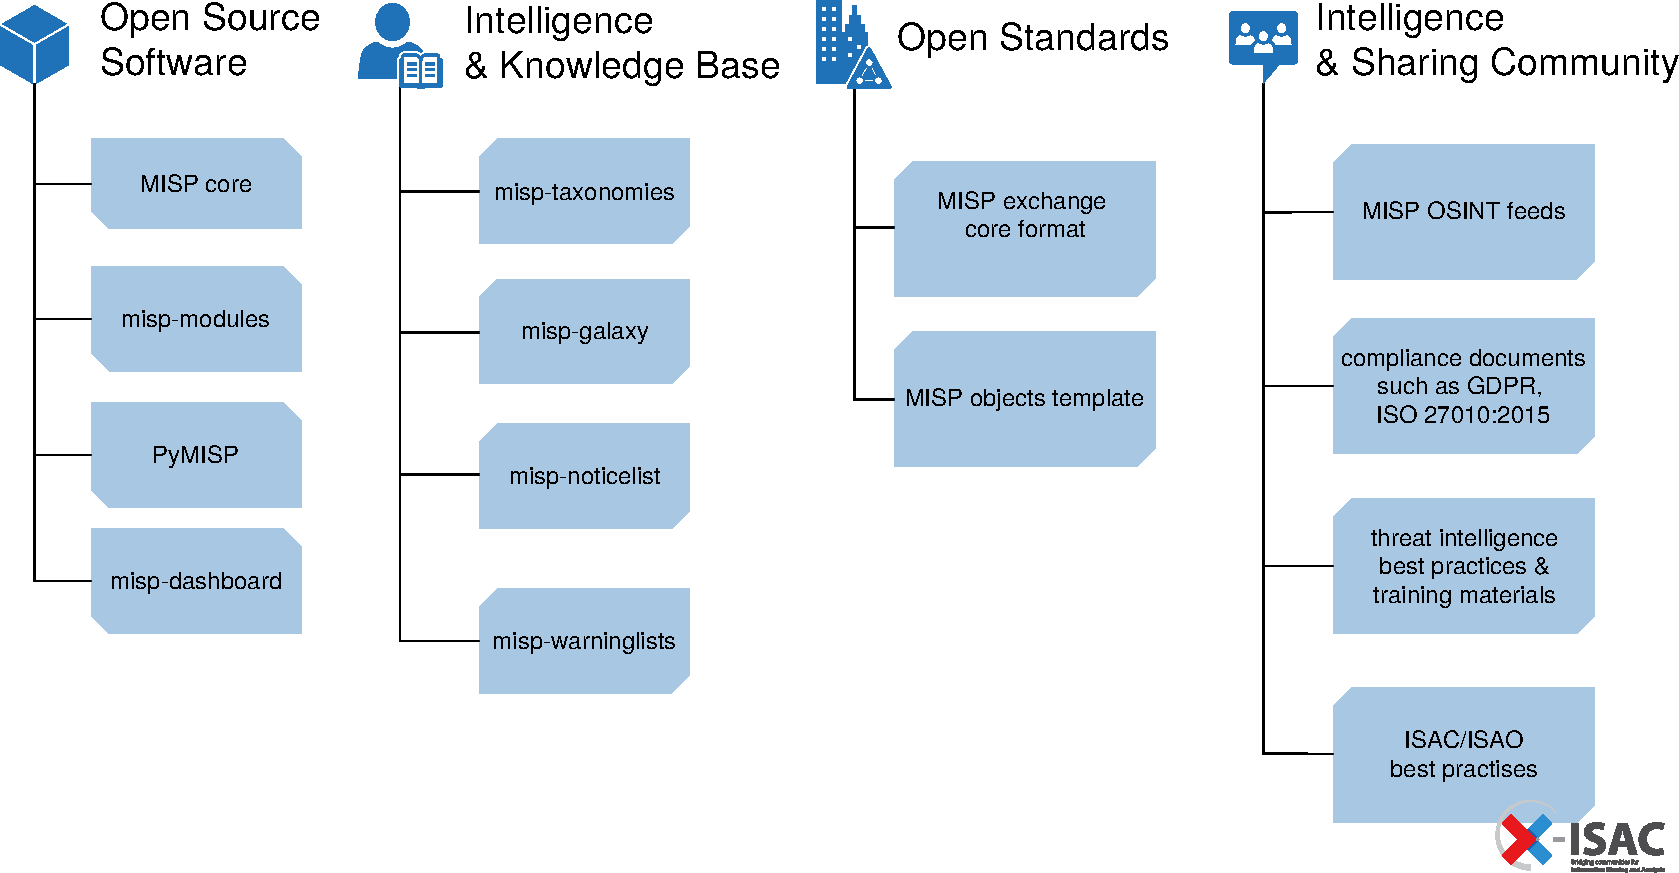
\includegraphics[scale=0.35]{misp-overview-simplified.pdf}
\end{frame}

\begin{frame}
        \frametitle{Helping Contributors in MISP}
        \begin{itemize}
            \item Contributors can use the UI, API or using the freetext import to add events and attributes.
                \begin{itemize}
                        \item Modules existing in Viper (a binary framework for malware reverser) to populate and use MISP from the vty or via your IDA.
                \end{itemize}
        \item Contribution can be direct by creating an event but {\bf users can propose attributes updates} to the event owner.
            \item {\bf Users should not be forced to use a single interface to contribute}.
        \end{itemize}
\end{frame}

\begin{frame}
        \frametitle{Getting some naming conventions out of the way...}
         \begin{itemize}
                \item Data layer
                \begin{itemize}
                    \item {\bf Events} are encapsulations for contextually linked information
                    \item {\bf Attributes} are individual data points, which can be indicators or supporting data.
                    \item {\bf Objects} are custom templated Attribute compositions
                    \item {\bf Object references} are the relationships between other building blocks
                \end{itemize}
                \item Context layer
                \begin{itemize}
                    \item {\bf Tags} are labels attached to events/attributes and can come from {\bf Taxonomies}
                    \item {\bf Galaxy-clusters} are knowledge base items used to label events/attributes and come from {\bf Galaxies}. 
                \end{itemize}
        \end{itemize}
\end{frame}

\begin{frame}
        \frametitle{A rich data-model: telling stories via relationships}
        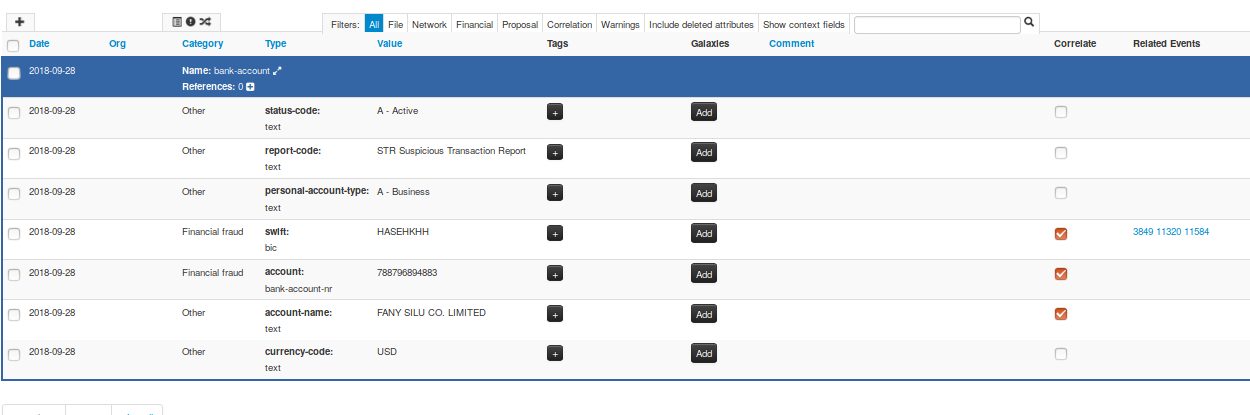
\includegraphics[scale=0.24]{screenshots/bankaccount.png}
        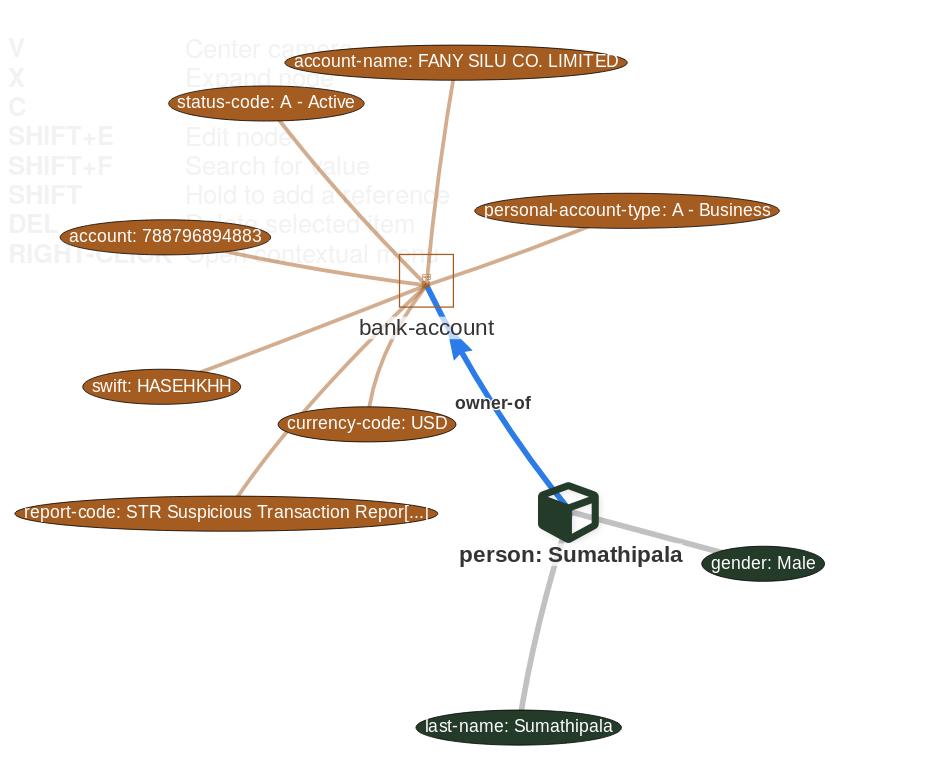
\includegraphics[scale=0.18]{screenshots/bankview.png}
\end{frame}

\begin{frame}
        \frametitle{Contextualisation and aggregation}
        \begin{itemize}
                \item MISP integrates at the event and the attribute levels MITRE's Adversarial Tactics, Techniques, and Common Knowledge (ATT\&CK).
        \end{itemize}
        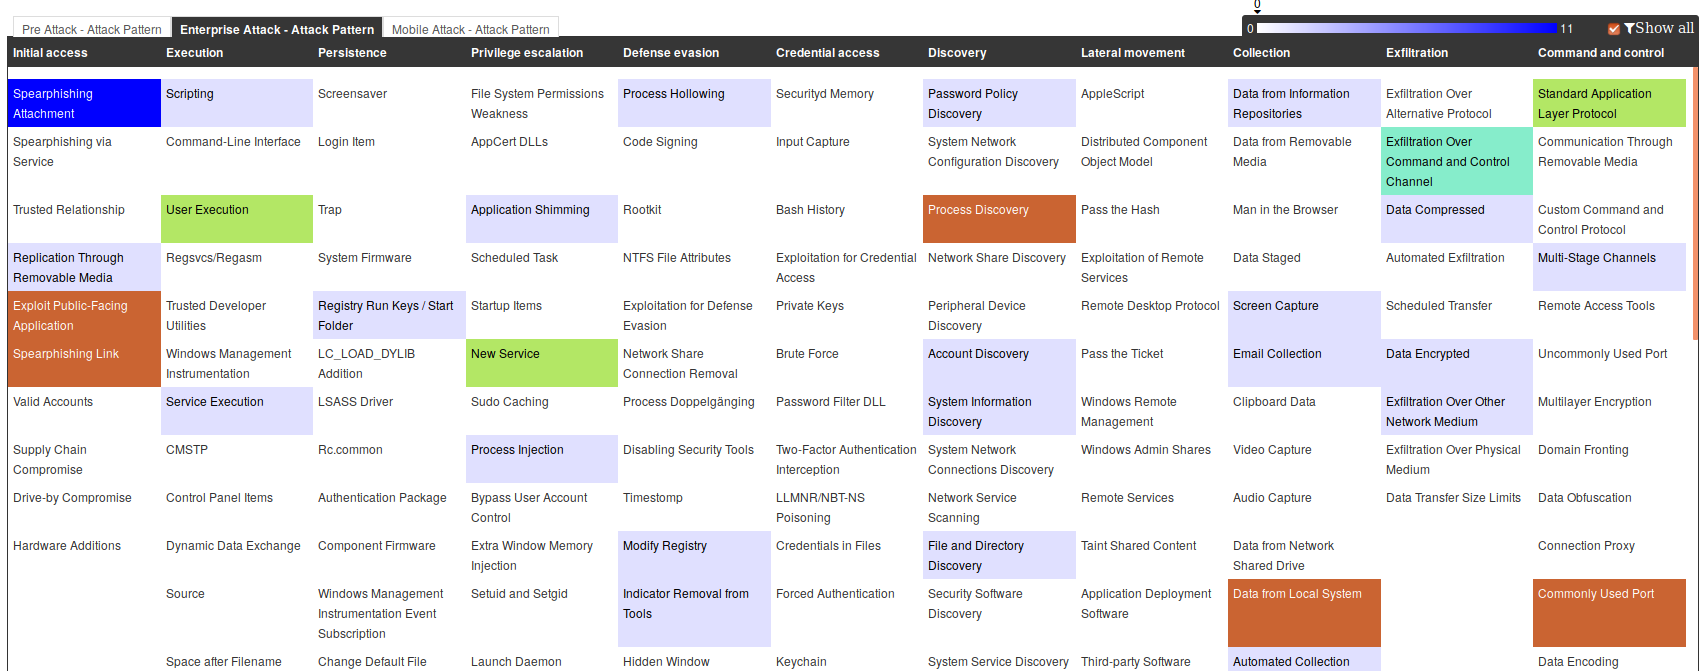
\includegraphics[scale=0.2]{screenshots/attack-screenshot.png}
\end{frame}

\begin{frame}
\frametitle{Sharing in MISP}
    \begin{itemize}
        \item Sharing via distribution lists - {\bf Sharing groups}
        \item {\bf Delegation} for pseudo-anonymised information sharing
        \item {\bf Proposals} and {\bf Extended events} for collaborated information sharing
        \item Synchronisation, Feed system, air-gapped sharing
        \item User defined {\bf filtered sharing} for all the above mentioned methods
        \item Cross-instance information {\bf caching} for quick lookups of large data-sets
        \item Support for multi-MISP internal enclaves
    \end{itemize}
\end{frame}

\begin{frame}
\frametitle{MISP core distributed sharing functionality}
\begin{itemize}
\item MISPs' core functionality is sharing where everyone can be a consumer and/or a contributor/producer."
\item Quick benefit without the obligation to contribute.
\item Low barrier access to get acquainted to the system.
\end{itemize}
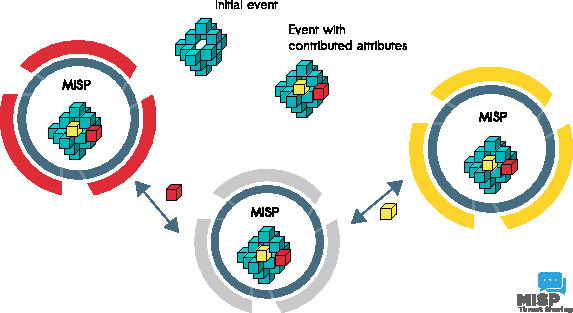
\includegraphics[scale=0.9]{misp-distributed.pdf}
\end{frame}



\begin{frame}
\frametitle{Information quality management}
    \begin{itemize}
        \item Correlating data
        \item Feedback loop from detections via {\bf Sightings}
        \item {\bf False positive management} via the warninglist system
        \item {\bf Enrichment system} via MISP-modules
        \item {\bf Integrations} with a plethora of tools and formats
        \item Flexible {\bf API} and support {\bf libraries} such as PyMISP to ease integration
        \item {\bf Timelines} and giving information a temporal context
        \item Full chain for {\bf indicator life-cycle management}
    \end{itemize}
\end{frame}

\begin{frame}
        \frametitle{Correlation features: a tool for analysts}
        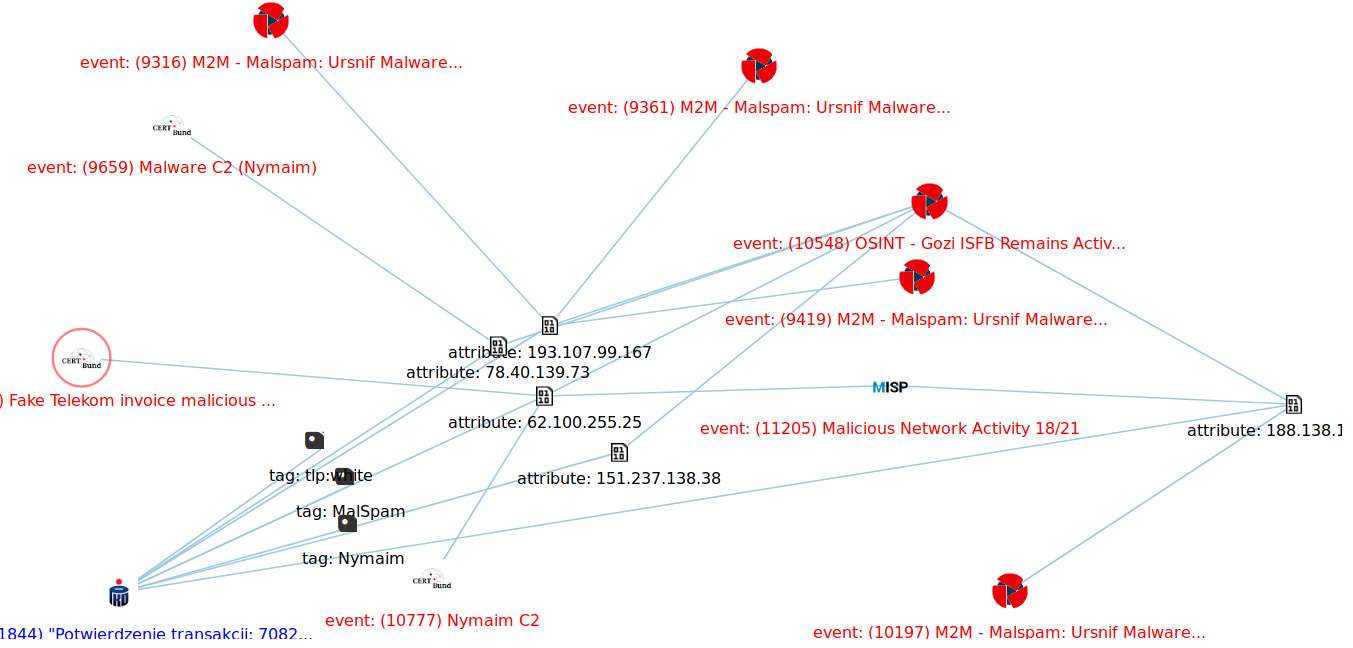
\includegraphics[scale=0.18]{screenshots/campaign.png}
        \begin{itemize}
                \item To {\bf corroborate a finding} (e.g. is this the same campaign?), {\bf reinforce an analysis} (e.g. do other analysts have the same hypothesis?), {\bf confirm a specific aspect} (e.g. are the sinkhole IP addresses used for one campaign?) or just find if this {\bf threat is new or unknown in your community}.
        \end{itemize}
\end{frame}

\begin{frame}
        \frametitle{Sightings support}
        \begin{columns}[t]
        \column{5.0cm}
        \begin{figure}
        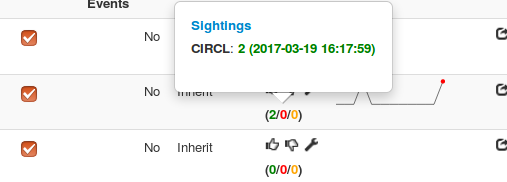
\includegraphics[scale=0.3]{screenshots/sighting-n.png}\\
        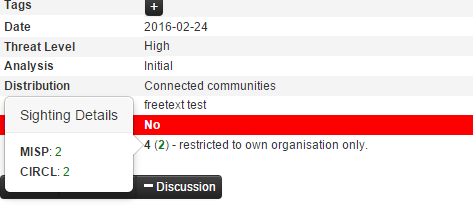
\includegraphics[scale=0.34]{screenshots/Sightings2.PNG}
        \end{figure}
        \column{7cm}
        \begin{itemize}
                \item Has a data-point been {\bf sighted} by me or the community before?
                \item Additionally, the sighting system supports negative sigthings (FP) and expiration sightings.
                \item Sightings can be performed via the API or the UI.
                \item Many use-cases for {\bf scoring indicators} based on users sighting.
                \item For large quantities of data, {\bf SightingDB} by Devo
        \end{itemize}
        \end{columns}
\end{frame}

\begin{frame}
  \frametitle{Timelines and giving information a temporal context}
  \begin{itemize}
    \item Recently introduced {\bf \texttt{first\_seen}} and {\bf \texttt{last\_seen}} data points
    \item All data-points can be placed in time
    \item Enables the {\bf visualisation} and {\bf adjustment} of indicators timeframes 
  \end{itemize}
  \begin{center}
    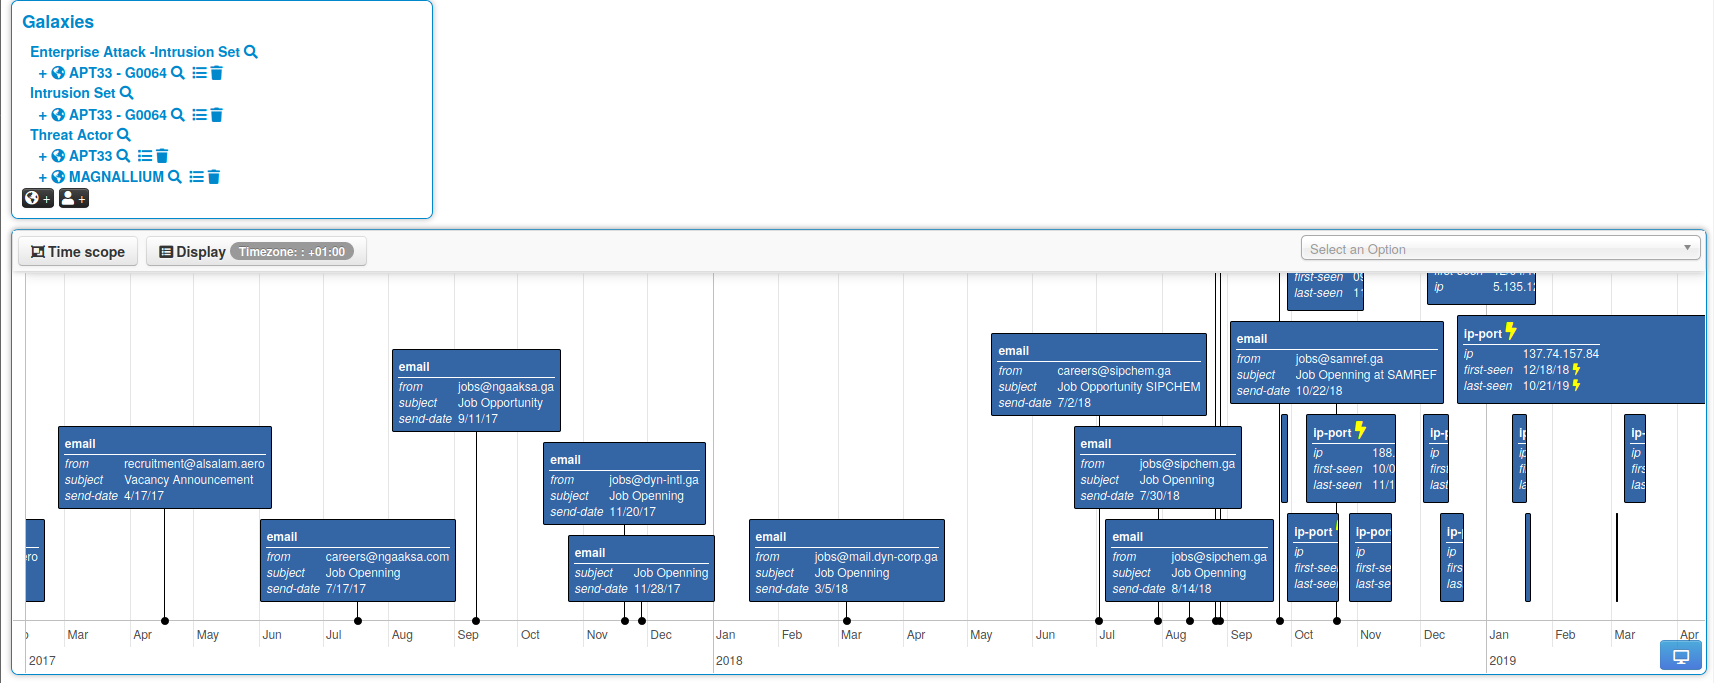
\includegraphics[width=1.0\linewidth]{timeline-misp-overview.png}
  \end{center}
\end{frame}

\begin{frame}
    \frametitle{Life-cycle management via decaying of indicators}
    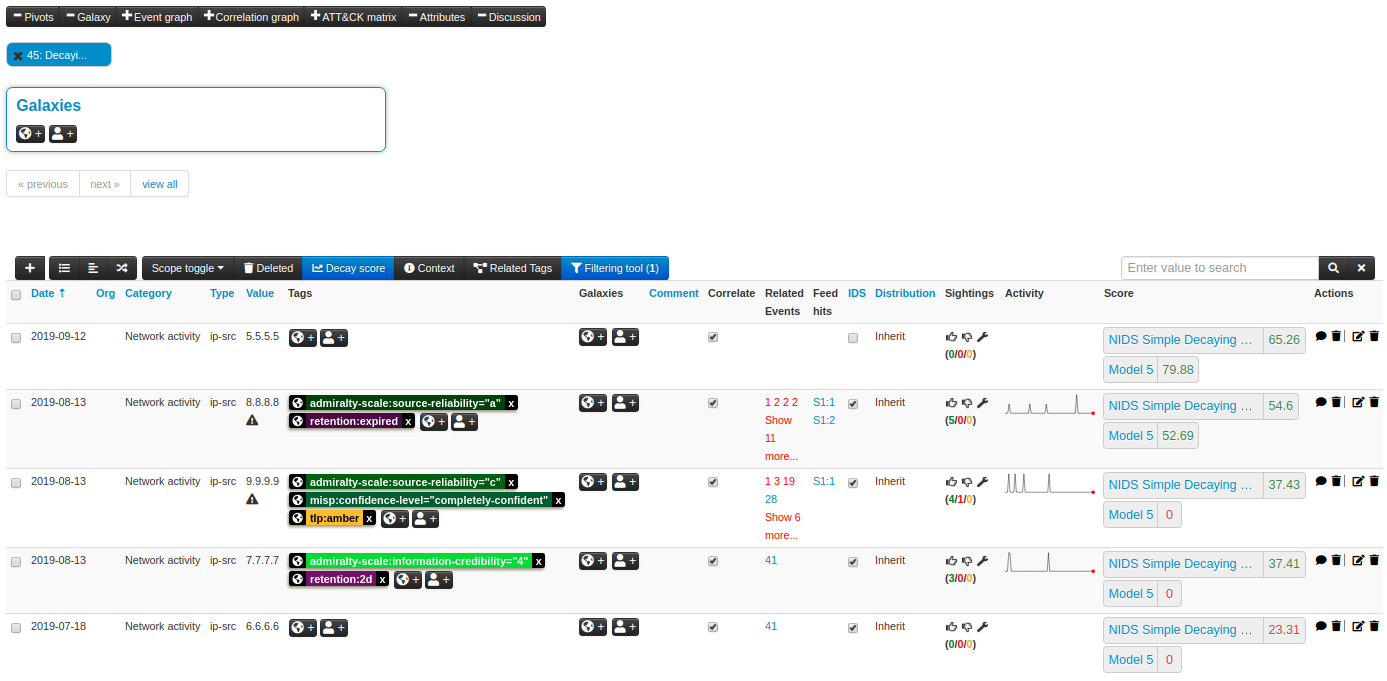
\includegraphics[width=1.00\linewidth]{decaying-event.png}
    \begin{itemize}
        \item \texttt{Decay score} toggle button
        \begin{itemize}
            \item Shows Score for each \textit{Models} associated to the \textit{Attribute} type
        \end{itemize}
    \end{itemize}
\end{frame}

\begin{frame}
    \frametitle{Decaying of indicators: Fine tuning tool}
    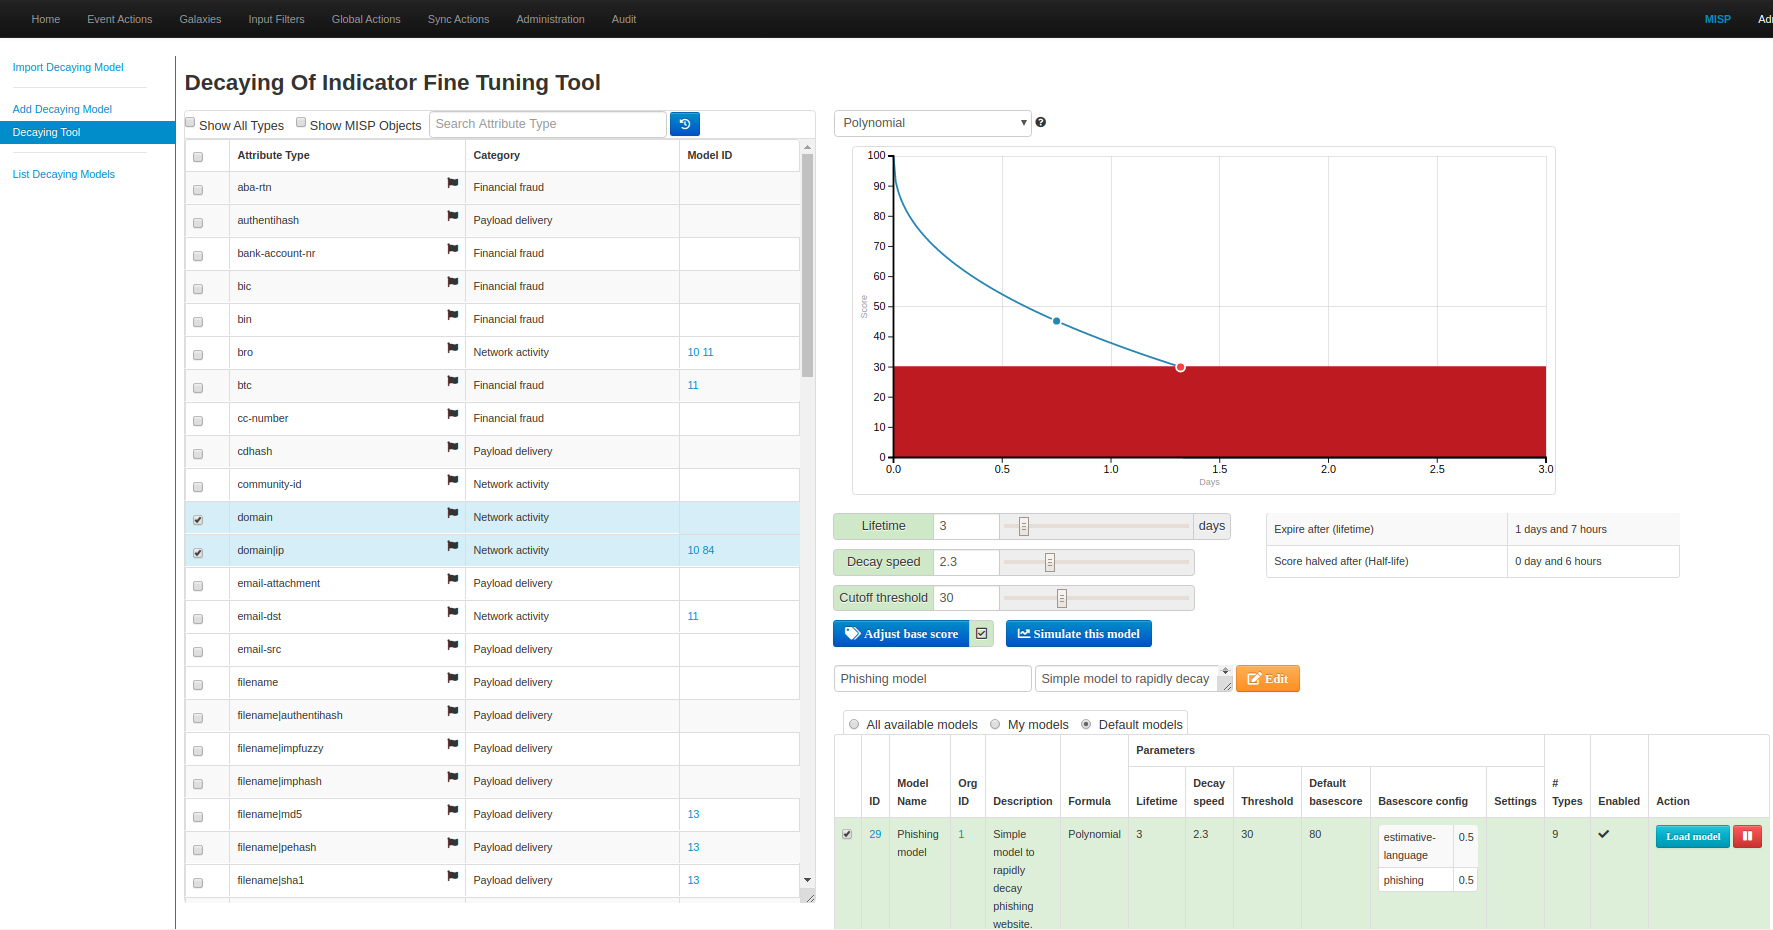
\includegraphics[width=1.00\linewidth]{decaying-tool.png}
    Create, modify, visualise, perform mapping
\end{frame}

\begin{frame}
    \frametitle{Decaying of indicators: simulation tool}
    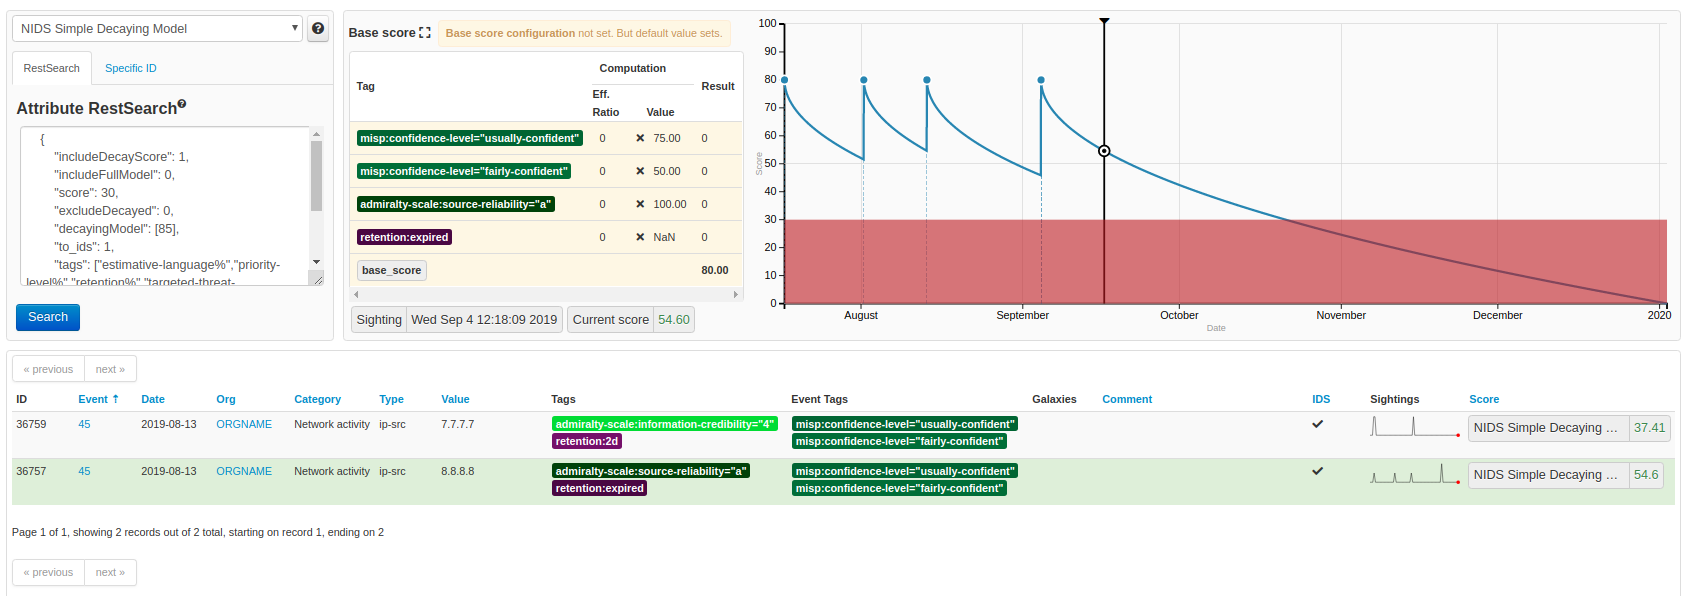
\includegraphics[width=1.00\linewidth]{decaying-simulation.png}
    Simulate \textit{Attributes} with different \textit{Models}
\end{frame}


\begin{frame}
        \frametitle{Conclusion}
        \begin{itemize}
                \item {\bf Information sharing practices come from usage} and by example (e.g. learning by imitation from the shared information).
                \item MISP is just a tool. What matters is your sharing practices. The tool should be as transparent as possible to support you.
                \item Enable users to customize MISP to meet their community's use-cases.
                \item MISP project combines open source software, open standards, best practices and communities to make information sharing a reality.
        \end{itemize}
\end{frame}

\begin{frame}
  \frametitle{Contact us}
  \begin{itemize}
    \item \url{https://www.misp-project.org/}
    \item \url{https://www.misp-standard.org/}
    \item \url{https://github.com/MISP}
    \item \url{info@misp-project.org}
    \item \url{https://twitter.com/MISPProject}
  \end{itemize}
\end{frame}


